\documentclass{beamer}
\usetheme{Antibes}
\usepackage{xcolor, colortbl}
\usepackage{algorithm}
\usepackage{algpseudocode}
\usepackage{textcomp}
\usepackage{listings}
\usepackage{hyperref}
\usepackage{alltt}
\usepackage{tikz}
\usepackage{framed}
\usepackage{marvosym}
\usepackage{wasysym}
\usepackage{marvosym}
\usepackage{crayola}
\usepackage{mathpartir}
\usepackage{tabularx}
\usepackage[belowskip=-15pt,aboveskip=0pt]{caption}
\usepackage[skins]{tcolorbox}
\usepackage{multicol}
\usetikzlibrary{positioning,shapes,arrows, arrows.meta, backgrounds, fit, shadows, automata}
\usetikzlibrary{decorations.markings, calc}
%\usepackage{wasysym}
%\usepackage{marvosym}
\setbeamertemplate{footline}[frame number]
%\usecolortheme{fly}
\usefonttheme{serif}

\title[Sujit]{Lexical Analysis \\
Programming Languages}
\author{Sujit Kumar Chakrabarti}
\institute{IIITB}
\date{}


\definecolor{lightblue}{rgb}{0.8,0.93,1.0} % color values Red, Green, Blue
\definecolor{darkblue}{rgb}{0.4,0.3,1.0} % color values Red, Green, Blue
\definecolor{Blue}{rgb}{0,0,1.0} % color values Red, Green, Blue
\definecolor{darkgreen}{rgb}{0,0.7,0.2} % color values Red, Green, Blue
\definecolor{Red}{rgb}{1,0,0} % color values Red, Green, Blue
\definecolor{Pink}{rgb}{0.7,0,0.2}
\definecolor{links}{HTML}{2A1B81}
\definecolor{mydarkgreen}{HTML}{126215}
\newcommand{\highlight}[1]{{\color{Red}(#1)}}

\newcommand{\myheader}[1]{
	{\color{darkblue}
		\begin{Large}
			\begin{center}
				{#1}
			\end{center}
		\end{Large}
	}
}
\newcommand{\myminorheader}[1]{
	{\color{BrickRed}
		\begin{Large}
			{\fontfamily{\sfdefault}\selectfont\textbf{#1}}
		\end{Large}
	}
}

%\tikzstyle{input} = [coordinate]
%\tikzstyle{output} = [coordinate]


\tikzstyle{bb}=[%
      rectangle, draw=black, thick, fill=OliveGreen!30, drop shadow, align=center,
      text ragged, minimum height=2em, minimum width=2em, inner sep=6pt
]

\tikzstyle{inv}=[%
      rectangle, draw=none,  align=center,
      text ragged, minimum height=2em, minimum width=2em, align=center, inner sep=6pt
]

\tikzstyle{db}=[%
      ellipse, draw=black, thick, fill=pink, drop shadow, align=center,
      text ragged, minimum height=2em, inner sep=6pt
]

\tikzstyle{jn}=[%
      inner sep=0cm, outer sep=0cm
]

\tikzstyle{io}=[%
      trapezium, trapezium left angle=60, trapezium right angle=120, draw=black, thick, fill=brown, drop shadow,
      text ragged, minimum height=2em, minimum width=2em, inner sep=6pt, align=center
]

\tikzstyle{glio}=[%
      trapezium, trapezium left angle=60, trapezium right angle=120, draw=red, line width = 1mm, fill=brown, drop shadow,
      text ragged, minimum height=2em, minimum width=2em, inner sep=6pt
]
\tikzstyle{gl}=[%
      rectangle, draw=red, line width = 1mm, fill=lightblue, drop shadow,
      text ragged, minimum height=2em, minimum width=2em, inner sep=6pt
]

\tikzstyle{en}=[%
      rectangle, draw=black, thick, fill=none,
      text ragged, minimum height=2em, minimum width=2em, inner sep=6pt
]

\tikzstyle{sh}=[%
      rectangle, draw=gray, thick, fill=none, color = gray,
      text ragged, minimum height=2em, minimum width=2em, inner sep=6pt
]

\tikzstyle{kcedge}=[%
      -{Latex[length=3mm,width=2mm]}, Red, thick
]

\lstdefinestyle{javacode}{
	language = Java,
	basicstyle = \ttfamily\scriptsize,
	stringstyle = \ttfamily,
	keywordstyle=\color{Blue}\bfseries,
	identifierstyle=\color{Pink},
	commentstyle=\color{darkgreen},
	frame=single,
	frameround=tttt,
%	numbers=left
	showstringspaces=false
}

\lstdefinestyle{camlcode}{
	language = Caml,
	basicstyle = \scriptsize\ttfamily,
	stringstyle = \color{red}\ttfamily,
	keywordstyle=\color{Blue}\bfseries,
	identifierstyle=\ttfamily,
	frame=single,
	frameround=tttt,
	numbers=none,
	showstringspaces=false,
	escapeinside={(*@}{@*)}
}

\lstdefinestyle{outputcode}{
	language = bash,
	backgroundcolor = \color{black},
	basicstyle = \tiny\ttfamily\color{white},
	stringstyle = \color{red}\ttfamily,
	keywordstyle=\color{white}\bfseries,
	identifierstyle=\ttfamily,
	frameround=tttt,
	numbers=none,
	showstringspaces=false,
	escapeinside={(*@}{@*)}
}

\newtcolorbox{myframe}[2][]{%
  enhanced,colback=white,colframe=black,coltitle=black,
  sharp corners,boxrule=0.4pt,
  fonttitle=\itshape,
  attach boxed title to top left={yshift=-0.3\baselineskip-0.4pt,xshift=2mm},
  boxed title style={tile,size=minimal,left=0.5mm,right=0.5mm,
    colback=white,before upper=\strut},
  title=#2,#1
}

\begin{document}
\maketitle

\section{Simulation of NFAs}

% frame begin %%%%%%%%%%%%%%%%%%%%%%%%
\begin{frame}{Non-Deterministic FSA (NFA)}
\begin{itemize}
	\item Finite set of states -- ($S$)
	\item Alphabet - ($\sum$)
	\item Transition function ($T : S \times \sum \rightarrow 2^S$)
	\item Initial state ($S_0$)
	\item Final/accepting states ($F \subseteq S$)
	\pause
	\item \textbf{Acceptance of a string: }When there exists a path corresponding to the input leading to an accepting state.
\end{itemize}

\end{frame}
% frame end %%%%%%%%%%%%%%%%%%%%%%%%

% frame begin %%%%%%%%%%%%%%%%%%%%%%%%
\begin{frame}{Simulation of NFAs}
{Salient Points}

\begin{itemize}
\item Possibly more than one outgoing transitions with the same label.
\item $\epsilon$-transitions
\item More than one paths can be traced during the same run.
\item All the possible traces have to be tracked.
\item Multiple states can be active at the same time.
\end{itemize}
\end{frame}
% frame end %%%%%%%%%%%%%%%%%%%%%%%%

% frame begin %%%%%%%%%%%%%%%%%%%%%%%%
\begin{frame}{Simulation of NFAs}
\myminorheader{Example 1}
\begin{center}
\resizebox{!}{0.2\textheight}{%
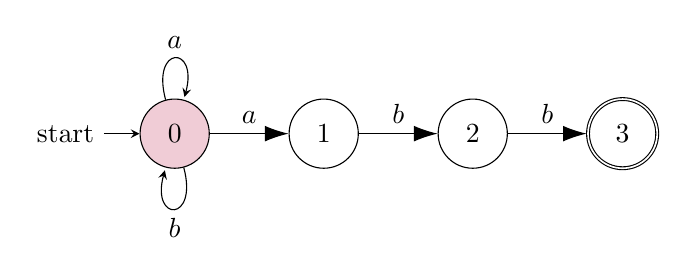
\begin{tikzpicture}[auto,
    -{Latex[length=3mm,width=2mm]},
    >=stealth
  ]
    \node[initial, state, fill=Pink!20]   (0)                {$0$};
    \node[state]            (1) [right = of 0] {$1$};
    \node[state] (2) [right = of 1] {$2$};
    \node[state, accepting] (3) [right = of 2] {$3$};
    
    \path (0) edge[-{Latex[length=3mm,width=2mm]}, loop above] node {$a$} (0)
          (0) edge[loop below] node {$b$} (0)
          (0) edge node {$a$} (1)
          (1) edge node {$b$} (2)
          (2) edge node {$b$} (3)
    ;

  \end{tikzpicture}
}

\vspace{1cm}
\begin{tabular}{p{0.3\textwidth} @{\hspace{1cm}} c}
\textbf{Input:} $aabbabb$ &
\resizebox{0.45\textwidth}{!}{
\begin{tikzpicture}
\node[circle, draw=Black] (s0) {0};
\node[circle, draw=none, above right=of s0] (s1) {\ };
\node[circle, draw=none, below right=of s1] (s2) {\ };
\node[circle, draw=none, right=of s2] (s3) {\ };
\node[circle, draw=none, right=of s3] (s4) {\ };
\node[circle, draw=none, above right=of s1] (s5) {\ };
\node[circle, draw=none, right=of s5] (s6) {\ };
\node[circle, draw=none, right=of s6] (s7) {\ };
\node[circle, draw=none, below right=of s7] (s8) {\ };
\node[circle, draw=none, right=of s8] (s9) {\ };
\node[circle, draw=none, right=of s9] (s10) {\ };
\node[circle, draw=none, above right=of s7] (s11) {\ };
\node[circle, draw=none, right=of s11] (s12) {\ };
\node[circle, draw=none, right=of s12] (s13) {\ };
\node[circle, draw=none, below right=of s0] (s14) {\ };

%\draw[->] (s0) to node[above]{a} (s1);
%\draw[->] (s1) to node[above]{a} (s2);
%\draw[->] (s2) to node[above]{b} (s3);
%\draw[->] (s3) to node[above]{b} (s4);
%\draw[->] (s1) to node[above]{a} (s5);
%\draw[->] (s5) to node[above]{b} (s6);
%\draw[->] (s6) to node[above]{b} (s7);
%\draw[->] (s7) to node[above]{a} (s8);
%\draw[->] (s8) to node[above]{b} (s9);
%\draw[->] (s9) to node[above]{b} (s10);
%\draw[->] (s7) to node[above]{a} (s11);
%\draw[->] (s11) to node[above]{b} (s12);
%\draw[->] (s12) to node[above]{b} (s13);
%\draw[->] (s0) to node[above]{b} (s14);

%\node[inv, right=0.1cm of s14](cross1){\Large\color{Red}\textbf{$\times$}};
%\node[inv, right=0.1cm of s4](cross2){\Large\color{Red}\textbf{$\times$}};
%\node[inv, right=0.1cm of s13](cross13){\Large\color{Red}\textbf{$\times$}};
%\node[inv, right=0.1cm of s10](cross1){\Large\color{Green}\textbf{\checkmark}};
\end{tikzpicture}
}
\end{tabular}

\end{center}

\end{frame}
% frame end %%%%%%%%%%%%%%%%%%%%%%%%

% frame begin %%%%%%%%%%%%%%%%%%%%%%%%
\begin{frame}{Simulation of NFAs}
\myminorheader{Example 1}
\begin{center}
\resizebox{!}{0.2\textheight}{%
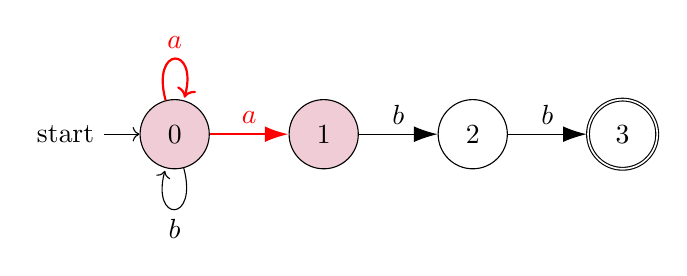
\begin{tikzpicture}[auto,
    ->,
    -{Latex[length=3mm,width=2mm]}
  ]
    \node[initial, state, fill=Pink!20]   (0)                {$0$};
    \node[state]            (1) [, fill=Pink!20, right = of 0] {$1$};
    \node[state] (2) [right = of 1] {$2$};
    \node[state, accepting] (3) [right = of 2] {$3$};
    
    \path (0) edge[Red, thick, loop above] node {$a$} (0)
          (0) edge[loop below] node {$b$} (0)
          (0) edge[Red, thick] node {$a$} (1)
          (1) edge node {$b$} (2)
          (2) edge node {$b$} (3)
    ;

  \end{tikzpicture}
}

\vspace{1cm}
\begin{tabular}{p{0.3\textwidth} @{\hspace{1cm}} c}
\textbf{Input:} ${\color{Red}\textbf{a}}abbabb$ &
\resizebox{0.45\textwidth}{!}{
\begin{tikzpicture}
\node[circle, draw=Black] (s0) {0};
\node[circle, draw=Black, above right=of s0] (s1) {0};
\node[circle, draw=none, below right=of s1] (s2) {\ };
\node[circle, draw=none, right=of s2] (s3) {\ };
\node[circle, draw=none, right=of s3] (s4) {\ };
\node[circle, draw=none, above right=of s1] (s5) {\ };
\node[circle, draw=none, right=of s5] (s6) {\ };
\node[circle, draw=none, right=of s6] (s7) {\ };
\node[circle, draw=none, below right=of s7] (s8) {\ };
\node[circle, draw=none, right=of s8] (s9) {\ };
\node[circle, draw=none, right=of s9] (s10) {\ };
\node[circle, draw=none, above right=of s7] (s11) {\ };
\node[circle, draw=none, right=of s11] (s12) {\ };
\node[circle, draw=none, right=of s12] (s13) {\ };
\node[circle, draw=Black, below right=of s0] (s14) {1};

\draw[->] (s0) to node[above]{a} (s1);
%\draw[->] (s1) to node[above]{a} (s2);
%\draw[->] (s2) to node[above]{b} (s3);
%\draw[->] (s3) to node[above]{b} (s4);
%\draw[->] (s1) to node[above]{a} (s5);
%\draw[->] (s5) to node[above]{b} (s6);
%\draw[->] (s6) to node[above]{b} (s7);
%\draw[->] (s7) to node[above]{a} (s8);
%\draw[->] (s8) to node[above]{b} (s9);
%\draw[->] (s9) to node[above]{b} (s10);
%\draw[->] (s7) to node[above]{a} (s11);
%\draw[->] (s11) to node[above]{b} (s12);
%\draw[->] (s12) to node[above]{b} (s13);
\draw[->] (s0) to node[above]{a} (s14);

%\node[inv, right=0.1cm of s14](cross1){\Large\color{Red}\textbf{$\times$}};
%\node[inv, right=0.1cm of s4](cross2){\Large\color{Red}\textbf{$\times$}};
%\node[inv, right=0.1cm of s13](cross13){\Large\color{Red}\textbf{$\times$}};
%\node[inv, right=0.1cm of s10](cross1){\Large\color{Green}\textbf{\checkmark}};
\end{tikzpicture}
}
\end{tabular}

\end{center}

\end{frame}
% frame end %%%%%%%%%%%%%%%%%%%%%%%%

% frame begin %%%%%%%%%%%%%%%%%%%%%%%%
\begin{frame}{Simulation of NFAs}
\myminorheader{Example 1}
\begin{center}
\resizebox{!}{0.2\textheight}{%
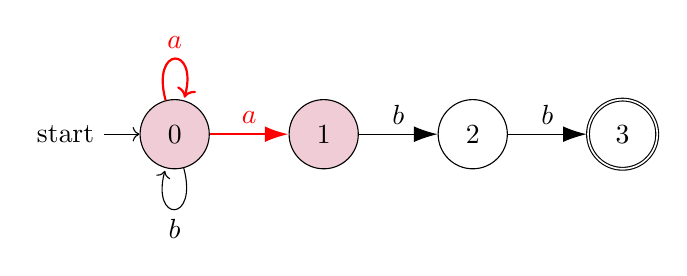
\begin{tikzpicture}[auto,
    ->,
    -{Latex[length=3mm,width=2mm]}
  ]
    \node[initial, state, fill=Pink!20]   (0)                {$0$};
    \node[state]            (1) [, fill=Pink!20, right = of 0] {$1$};
    \node[state] (2) [right = of 1] {$2$};
    \node[state, accepting] (3) [right = of 2] {$3$};
    
    \path (0) edge[Red, thick, loop above] node {$a$} (0)
          (0) edge[loop below] node {$b$} (0)
          (0) edge[Red, thick] node {$a$} (1)
          (1) edge node {$b$} (2)
          (2) edge node {$b$} (3)
    ;

  \end{tikzpicture}
}

\vspace{1cm}
\begin{tabular}{p{0.3\textwidth} @{\hspace{1cm}} c}
\textbf{Input:} $a{\color{Red}\textbf{a}}bbabb$ &
\resizebox{0.45\textwidth}{!}{
\begin{tikzpicture}
\node[circle, draw=Black] (s0) {0};
\node[circle, draw=Black, above right=of s0] (s1) {0};
\node[circle, draw=Black, below right=of s1] (s2) {1};
\node[circle, draw=none, right=of s2] (s3) {\ };
\node[circle, draw=none, right=of s3] (s4) {\ };
\node[circle, draw=Black, above right=of s1] (s5) {0};
\node[circle, draw=none, right=of s5] (s6) {\ };
\node[circle, draw=none, right=of s6] (s7) {\ };
\node[circle, draw=none, below right=of s7] (s8) {\ };
\node[circle, draw=none, right=of s8] (s9) {\ };
\node[circle, draw=none, right=of s9] (s10) {\ };
\node[circle, draw=none, above right=of s7] (s11) {\ };
\node[circle, draw=none, right=of s11] (s12) {\ };
\node[circle, draw=none, right=of s12] (s13) {\ };
\node[circle, draw=Black, below right=of s0] (s14) {1};

\draw[->] (s0) to node[above]{a} (s1);
\draw[->] (s1) to node[above]{a} (s2);
%\draw[->] (s2) to node[above]{b} (s3);
%\draw[->] (s3) to node[above]{b} (s4);
\draw[->] (s1) to node[above]{a} (s5);
%\draw[->] (s5) to node[above]{b} (s6);
%\draw[->] (s6) to node[above]{b} (s7);
%\draw[->] (s7) to node[above]{a} (s8);
%\draw[->] (s8) to node[above]{b} (s9);
%\draw[->] (s9) to node[above]{b} (s10);
%\draw[->] (s7) to node[above]{a} (s11);
%\draw[->] (s11) to node[above]{b} (s12);
%\draw[->] (s12) to node[above]{b} (s13);
\draw[->] (s0) to node[above]{a} (s14);

\node[inv, right=0.1cm of s14](cross1){\Large\color{Red}\textbf{$\times$}};
%\node[inv, right=0.1cm of s4](cross2){\Large\color{Red}\textbf{$\times$}};
%\node[inv, right=0.1cm of s13](cross13){\Large\color{Red}\textbf{$\times$}};
%\node[inv, right=0.1cm of s10](cross1){\Large\color{Green}\textbf{\checkmark}};
\end{tikzpicture}
}
\end{tabular}

\end{center}

\end{frame}
% frame end %%%%%%%%%%%%%%%%%%%%%%%%

% frame begin %%%%%%%%%%%%%%%%%%%%%%%%
\begin{frame}{Simulation of NFAs}
\myminorheader{Example 1}
\begin{center}
\resizebox{!}{0.2\textheight}{%
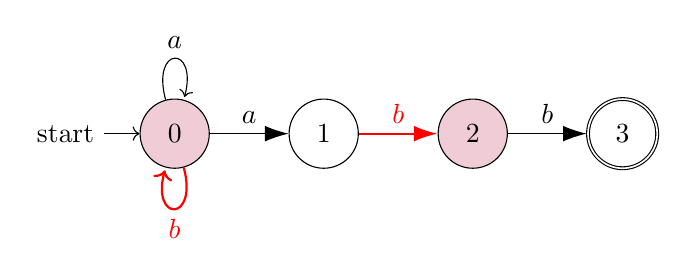
\begin{tikzpicture}[auto,
    ->,
    -{Latex[length=3mm,width=2mm]}
  ]
    \node[initial, state, fill=Pink!20]   (0)                {$0$};
    \node[state]            (1) [right = of 0] {$1$};
    \node[state] (2) [fill=Pink!20, right = of 1] {$2$};
    \node[state, accepting] (3) [right = of 2] {$3$};
    
    \path (0) edge[loop above] node {$a$} (0)
          (0) edge[Red, thick, loop below] node {$b$} (0)
          (0) edge node {$a$} (1)
          (1) edge[Red, thick] node {$b$} (2)
          (2) edge node {$b$} (3)
    ;

  \end{tikzpicture}
}

\vspace{1cm}
\begin{tabular}{p{0.3\textwidth} @{\hspace{1cm}} c}
\textbf{Input:} $aa{\color{Red}\textbf{b}}babb$ &
\resizebox{0.45\textwidth}{!}{
\begin{tikzpicture}
\node[circle, draw=Black] (s0) {0};
\node[circle, draw=Black, above right=of s0] (s1) {0};
\node[circle, draw=Black, below right=of s1] (s2) {1};
\node[circle, draw=Black, right=of s2] (s3) {2};
\node[circle, draw=none, right=of s3] (s4) {\ };
\node[circle, draw=Black, above right=of s1] (s5) {0};
\node[circle, draw=Black, right=of s5] (s6) {0};
\node[circle, draw=none, right=of s6] (s7) {\ };
\node[circle, draw=none, below right=of s7] (s8) {\ };
\node[circle, draw=none, right=of s8] (s9) {\ };
\node[circle, draw=none, right=of s9] (s10) {\ };
\node[circle, draw=none, above right=of s7] (s11) {\ };
\node[circle, draw=none, right=of s11] (s12) {\ };
\node[circle, draw=none, right=of s12] (s13) {\ };
\node[circle, draw=Black, below right=of s0] (s14) {1};

\draw[->] (s0) to node[above]{a} (s1);
\draw[->] (s1) to node[above]{a} (s2);
\draw[->] (s2) to node[above]{b} (s3);
%\draw[->] (s3) to node[above]{b} (s4);
\draw[->] (s1) to node[above]{a} (s5);
\draw[->] (s5) to node[above]{b} (s6);
%\draw[->] (s6) to node[above]{b} (s7);
%\draw[->] (s7) to node[above]{a} (s8);
%\draw[->] (s8) to node[above]{b} (s9);
%\draw[->] (s9) to node[above]{b} (s10);
%\draw[->] (s7) to node[above]{a} (s11);
%\draw[->] (s11) to node[above]{b} (s12);
%\draw[->] (s12) to node[above]{b} (s13);
\draw[->] (s0) to node[above]{a} (s14);

\node[inv, right=0.1cm of s14](cross1){\Large\color{Red}\textbf{$\times$}};
%\node[inv, right=0.1cm of s4](cross2){\Large\color{Red}\textbf{$\times$}};
%\node[inv, right=0.1cm of s13](cross13){\Large\color{Red}\textbf{$\times$}};
%\node[inv, right=0.1cm of s10](cross1){\Large\color{Green}\textbf{\checkmark}};
\end{tikzpicture}
}
\end{tabular}

\end{center}

\end{frame}
% frame end %%%%%%%%%%%%%%%%%%%%%%%%

% frame begin %%%%%%%%%%%%%%%%%%%%%%%%
\begin{frame}{Simulation of NFAs}
\myminorheader{Example 1}
\begin{center}
\resizebox{!}{0.2\textheight}{%
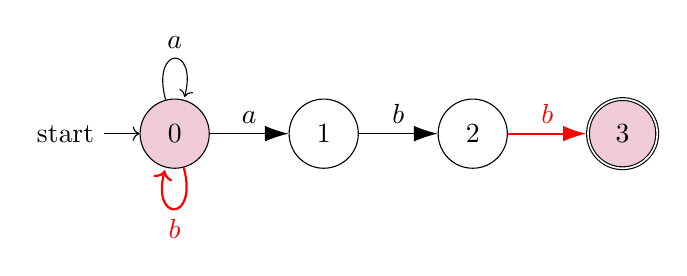
\begin{tikzpicture}[auto,
    ->,
    -{Latex[length=3mm,width=2mm]}
  ]
    \node[initial, state, fill=Pink!20]   (0)                {$0$};
    \node[state]            (1) [right = of 0] {$1$};
    \node[state] (2) [right = of 1] {$2$};
    \node[state, accepting] (3) [fill=Pink!20, right = of 2] {$3$};
    
    \path (0) edge[loop above] node {$a$} (0)
          (0) edge[Red, thick, loop below] node {$b$} (0)
          (0) edge node {$a$} (1)
          (1) edge node {$b$} (2)
          (2) edge[Red, thick] node {$b$} (3)
    ;

  \end{tikzpicture}
}

\vspace{1cm}
\begin{tabular}{p{0.3\textwidth} @{\hspace{1cm}} c}
\textbf{Input:} $aab{\color{Red}\textbf{b}}abb$ &
\resizebox{0.45\textwidth}{!}{
\begin{tikzpicture}
\node[circle, draw=Black] (s0) {0};
\node[circle, draw=Black, above right=of s0] (s1) {0};
\node[circle, draw=Black, below right=of s1] (s2) {1};
\node[circle, draw=Black, right=of s2] (s3) {2};
\node[circle, draw=Black, right=of s3] (s4) {3};
\node[circle, draw=Black, above right=of s1] (s5) {0};
\node[circle, draw=Black, right=of s5] (s6) {0};
\node[circle, draw=Black, right=of s6] (s7) {0};
\node[circle, draw=none, below right=of s7] (s8) {\ };
\node[circle, draw=none, right=of s8] (s9) {\ };
\node[circle, draw=none, right=of s9] (s10) {\ };
\node[circle, draw=none, above right=of s7] (s11) {\ };
\node[circle, draw=none, right=of s11] (s12) {\ };
\node[circle, draw=none, right=of s12] (s13) {\ };
\node[circle, draw=Black, below right=of s0] (s14) {1};

\draw[->] (s0) to node[above]{a} (s1);
\draw[->] (s1) to node[above]{a} (s2);
\draw[->] (s2) to node[above]{b} (s3);
\draw[->] (s3) to node[above]{b} (s4);
\draw[->] (s1) to node[above]{a} (s5);
\draw[->] (s5) to node[above]{b} (s6);
\draw[->] (s6) to node[above]{b} (s7);
%\draw[->] (s7) to node[above]{a} (s8);
%\draw[->] (s8) to node[above]{b} (s9);
%\draw[->] (s9) to node[above]{b} (s10);
%\draw[->] (s7) to node[above]{a} (s11);
%\draw[->] (s11) to node[above]{b} (s12);
%\draw[->] (s12) to node[above]{b} (s13);
\draw[->] (s0) to node[above]{a} (s14);

\node[inv, right=0.1cm of s14](cross1){\Large\color{Red}\textbf{$\times$}};
%\node[inv, right=0.1cm of s4](cross2){\Large\color{Red}\textbf{$\times$}};
%\node[inv, right=0.1cm of s13](cross13){\Large\color{Red}\textbf{$\times$}};
%\node[inv, right=0.1cm of s10](cross1){\Large\color{Green}\textbf{\checkmark}};
\end{tikzpicture}
}
\end{tabular}

\end{center}

\end{frame}
% frame end %%%%%%%%%%%%%%%%%%%%%%%%

% frame begin %%%%%%%%%%%%%%%%%%%%%%%%
\begin{frame}{Simulation of NFAs}
\myminorheader{Example 1}
\begin{center}
\resizebox{!}{0.2\textheight}{%
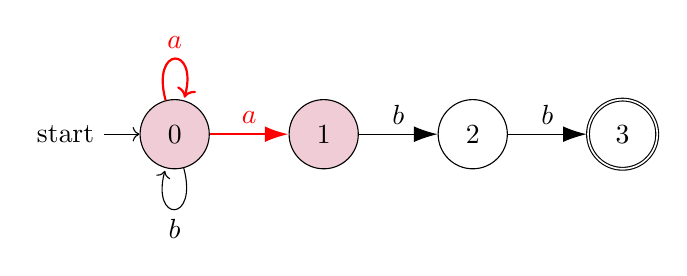
\begin{tikzpicture}[auto,
    ->,
    -{Latex[length=3mm,width=2mm]}
  ]
    \node[initial, state, fill=Pink!20]   (0)                {$0$};
    \node[state, fill=Pink!20]            (1) [right = of 0] {$1$};
    \node[state] (2) [right = of 1] {$2$};
    \node[state, accepting] (3) [right = of 2] {$3$};
    
    \path (0) edge[Red, thick, loop above] node {$a$} (0)
          (0) edge[loop below] node {$b$} (0)
          (0) edge[Red, thick] node {$a$} (1)
          (1) edge node {$b$} (2)
          (2) edge node {$b$} (3)
    ;

  \end{tikzpicture}
}

\vspace{1cm}
\begin{tabular}{p{0.3\textwidth} @{\hspace{1cm}} c}
\textbf{Input:} $aabb{\color{Red}\textbf{a}}bb$ &
\resizebox{0.45\textwidth}{!}{
\begin{tikzpicture}
\node[circle, draw=Black] (s0) {0};
\node[circle, draw=Black, above right=of s0] (s1) {0};
\node[circle, draw=Black, below right=of s1] (s2) {1};
\node[circle, draw=Black, right=of s2] (s3) {2};
\node[circle, draw=Black, right=of s3] (s4) {3};
\node[circle, draw=Black, above right=of s1] (s5) {0};
\node[circle, draw=Black, right=of s5] (s6) {0};
\node[circle, draw=Black, right=of s6] (s7) {0};
\node[circle, draw=Black, below right=of s7] (s8) {1};
\node[circle, draw=none, right=of s8] (s9) {\ };
\node[circle, draw=none, right=of s9] (s10) {\ };
\node[circle, draw=Black, above right=of s7] (s11) {0};
\node[circle, draw=none, right=of s11] (s12) {\ };
\node[circle, draw=none, right=of s12] (s13) {\ };
\node[circle, draw=Black, below right=of s0] (s14) {1};

\draw[->] (s0) to node[above]{a} (s1);
\draw[->] (s1) to node[above]{a} (s2);
\draw[->] (s2) to node[above]{b} (s3);
\draw[->] (s3) to node[above]{b} (s4);
\draw[->] (s1) to node[above]{a} (s5);
\draw[->] (s5) to node[above]{b} (s6);
\draw[->] (s6) to node[above]{b} (s7);
\draw[->] (s7) to node[above]{a} (s8);
%\draw[->] (s8) to node[above]{b} (s9);
%\draw[->] (s9) to node[above]{b} (s10);
\draw[->] (s7) to node[above]{a} (s11);
%\draw[->] (s11) to node[above]{b} (s12);
%\draw[->] (s12) to node[above]{b} (s13);
\draw[->] (s0) to node[above]{a} (s14);

\node[inv, right=0.1cm of s14](cross1){\Large\color{Red}\textbf{$\times$}};
\node[inv, right=0.1cm of s4](cross2){\Large\color{Red}\textbf{$\times$}};
%\node[inv, right=0.1cm of s13](cross13){\Large\color{Red}\textbf{$\times$}};
%\node[inv, right=0.1cm of s10](cross1){\Large\color{Green}\textbf{\checkmark}};
\end{tikzpicture}
}
\end{tabular}

\end{center}

\end{frame}
% frame end %%%%%%%%%%%%%%%%%%%%%%%%

% frame begin %%%%%%%%%%%%%%%%%%%%%%%%
\begin{frame}{Simulation of NFAs}
\myminorheader{Example 1}
\begin{center}
\resizebox{!}{0.2\textheight}{%
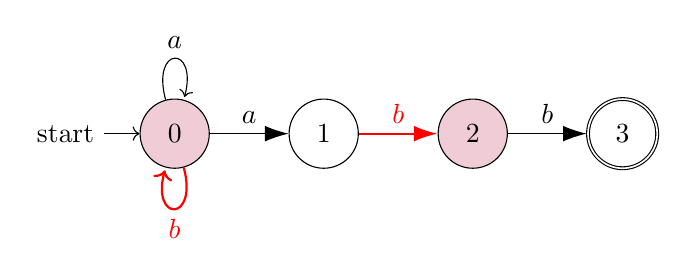
\begin{tikzpicture}[auto,
    ->,
    -{Latex[length=3mm,width=2mm]}
  ]
    \node[initial, state, fill=Pink!20]   (0)                {$0$};
    \node[state]            (1) [right = of 0] {$1$};
    \node[state, fill=Pink!20] (2) [right = of 1] {$2$};
    \node[state, accepting] (3) [right = of 2] {$3$};
    
    \path (0) edge[loop above] node {$a$} (0)
          (0) edge[Red, thick, loop below] node {$b$} (0)
          (0) edge node {$a$} (1)
          (1) edge[Red, thick] node {$b$} (2)
          (2) edge node {$b$} (3)
    ;

  \end{tikzpicture}
}

\vspace{1cm}
\begin{tabular}{p{0.3\textwidth} @{\hspace{1cm}} c}
\textbf{Input:} $aabba{\color{Red}\textbf{b}}b$ &
\resizebox{0.45\textwidth}{!}{
\begin{tikzpicture}
\node[circle, draw=Black] (s0) {0};
\node[circle, draw=Black, above right=of s0] (s1) {0};
\node[circle, draw=Black, below right=of s1] (s2) {1};
\node[circle, draw=Black, right=of s2] (s3) {2};
\node[circle, draw=Black, right=of s3] (s4) {3};
\node[circle, draw=Black, above right=of s1] (s5) {0};
\node[circle, draw=Black, right=of s5] (s6) {0};
\node[circle, draw=Black, right=of s6] (s7) {0};
\node[circle, draw=Black, below right=of s7] (s8) {1};
\node[circle, draw=Black, right=of s8] (s9) {2};
\node[circle, draw=none, right=of s9] (s10) {\ };
\node[circle, draw=Black, above right=of s7] (s11) {0};
\node[circle, draw=Black, right=of s11] (s12) {0};
\node[circle, draw=none, right=of s12] (s13) {\ };
\node[circle, draw=Black, below right=of s0] (s14) {1};

\draw[->] (s0) to node[above]{a} (s1);
\draw[->] (s1) to node[above]{a} (s2);
\draw[->] (s2) to node[above]{b} (s3);
\draw[->] (s3) to node[above]{b} (s4);
\draw[->] (s1) to node[above]{a} (s5);
\draw[->] (s5) to node[above]{b} (s6);
\draw[->] (s6) to node[above]{b} (s7);
\draw[->] (s7) to node[above]{a} (s8);
\draw[->] (s8) to node[above]{b} (s9);
%\draw[->] (s9) to node[above]{b} (s10);
\draw[->] (s7) to node[above]{a} (s11);
\draw[->] (s11) to node[above]{b} (s12);
%\draw[->] (s12) to node[above]{b} (s13);
\draw[->] (s0) to node[above]{a} (s14);

\node[inv, right=0.1cm of s14](cross1){\Large\color{Red}\textbf{$\times$}};
\node[inv, right=0.1cm of s4](cross2){\Large\color{Red}\textbf{$\times$}};
%\node[inv, right=0.1cm of s13](cross13){\Large\color{Red}\textbf{$\times$}};
%\node[inv, right=0.1cm of s10](cross1){\Large\color{Green}\textbf{\checkmark}};
\end{tikzpicture}
}
\end{tabular}

\end{center}

\end{frame}
% frame end %%%%%%%%%%%%%%%%%%%%%%%%

% frame begin %%%%%%%%%%%%%%%%%%%%%%%%
\begin{frame}{Simulation of NFAs}
\myminorheader{Example 1}
\begin{center}
\resizebox{!}{0.2\textheight}{%
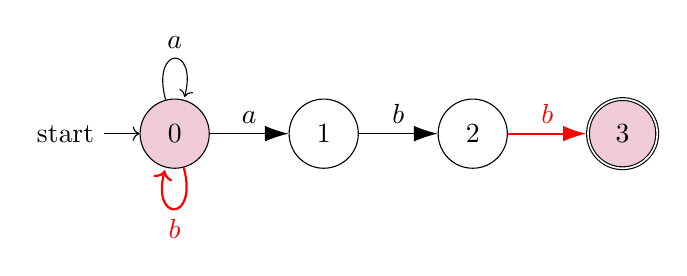
\begin{tikzpicture}[auto,
    ->,
    -{Latex[length=3mm,width=2mm]}
  ]
    \node[initial, state, fill=Pink!20]   (0)                {$0$};
    \node[state]            (1) [right = of 0] {$1$};
    \node[state] (2) [right = of 1] {$2$};
    \node[state, accepting, fill=Pink!20] (3) [right = of 2] {$3$};
    
    \path (0) edge[loop above] node {$a$} (0)
          (0) edge[Red, thick, loop below] node {$b$} (0)
          (0) edge node {$a$} (1)
          (1) edge node {$b$} (2)
          (2) edge[Red, thick] node {$b$} (3)
    ;

  \end{tikzpicture}
}

\vspace{1cm}
\begin{tabular}{p{0.3\textwidth} @{\hspace{1cm}} c}
\textbf{Input:} $aabbab{\color{Red}\textbf{b}}$ &
\resizebox{0.45\textwidth}{!}{
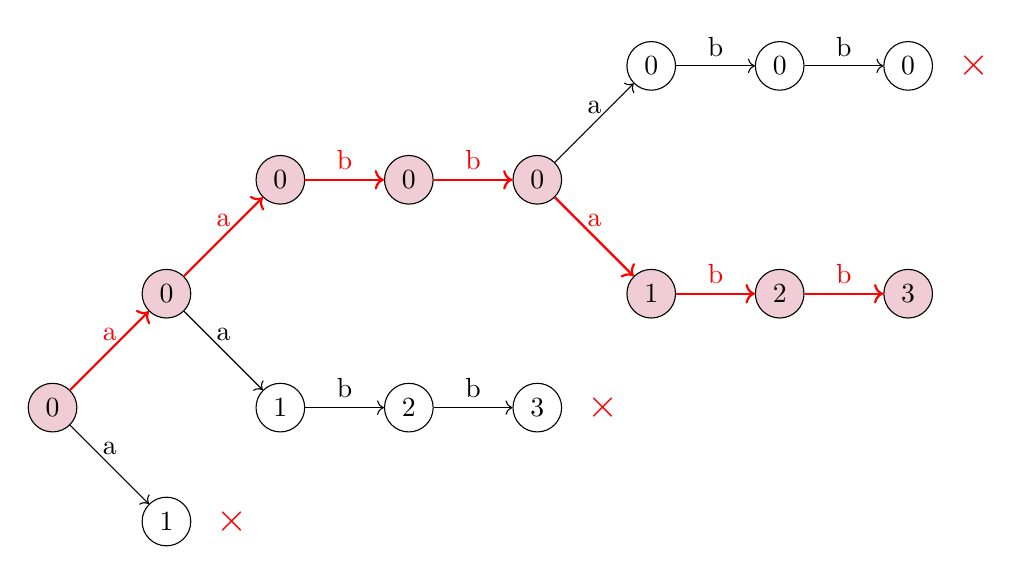
\begin{tikzpicture}
\node[circle, draw=Black, fill=Pink!20] (s0) {0};
\node[circle, draw=Black, fill=Pink!20, above right=of s0] (s1) {0};
\node[circle, draw=Black, below right=of s1] (s2) {1};
\node[circle, draw=Black, right=of s2] (s3) {2};
\node[circle, draw=Black, right=of s3] (s4) {3};
\node[circle, draw=Black, fill=Pink!20, above right=of s1] (s5) {0};
\node[circle, draw=Black, fill=Pink!20, right=of s5] (s6) {0};
\node[circle, draw=Black, fill=Pink!20, right=of s6] (s7) {0};
\node[circle, draw=Black, fill=Pink!20, below right=of s7] (s8) {1};
\node[circle, draw=Black, fill=Pink!20, right=of s8] (s9) {2};
\node[circle, draw=Black, fill=Pink!20, right=of s9] (s10) {3};
\node[circle, draw=Black, above right=of s7] (s11) {0};
\node[circle, draw=Black, right=of s11] (s12) {0};
\node[circle, draw=Black, right=of s12] (s13) {0};
\node[circle, draw=Black, below right=of s0] (s14) {1};

\draw[->, red, thick] (s0) to node[above]{a} (s1);
\draw[->] (s1) to node[above]{a} (s2);
\draw[->] (s2) to node[above]{b} (s3);
\draw[->] (s3) to node[above]{b} (s4);
\draw[->, red, thick] (s1) to node[above]{a} (s5);
\draw[->, red, thick] (s5) to node[above]{b} (s6);
\draw[->, red, thick] (s6) to node[above]{b} (s7);
\draw[->, red, thick] (s7) to node[above]{a} (s8);
\draw[->, red, thick] (s8) to node[above]{b} (s9);
\draw[->, red, thick] (s9) to node[above]{b} (s10);
\draw[->] (s7) to node[above]{a} (s11);
\draw[->] (s11) to node[above]{b} (s12);
\draw[->] (s12) to node[above]{b} (s13);
\draw[->] (s0) to node[above]{a} (s14);

\node[inv, right=0.1cm of s14](cross1){\Large\color{Red}\textbf{$\times$}};
\node[inv, right=0.1cm of s4](cross2){\Large\color{Red}\textbf{$\times$}};
\node[inv, right=0.1cm of s13](cross13){\Large\color{Red}\textbf{$\times$}};
\node[inv, right=0.1cm of s10](cross1){\Large\color{Green}\textbf{\checkmark}};
\end{tikzpicture}
}
\end{tabular}

\end{center}

\end{frame}
% frame end %%%%%%%%%%%%%%%%%%%%%%%%

% frame begin %%%%%%%%%%%%%%%%%%%%%%%%
\begin{frame}{Simulation of NFAs}
\myminorheader{Example 2.1}
\begin{center}
\resizebox{!}{0.35\textheight}{%
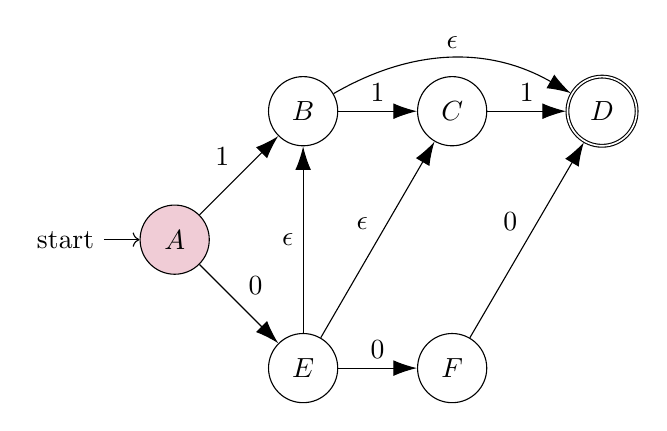
\begin{tikzpicture}[auto,
    ->,
    -{Latex[length=3mm,width=2mm]}
  ]
    \node[initial, state, fill=Pink!20]   (a)                {$A$};
    \node[state] (b) [above right = of a] {$B$};
    \node[state] (c) [right = of b] {$C$};
    \node[state, accepting] (d) [right = of c] {$D$};
    \node[state] (e) [below right = of a] {$E$};
    \node[state] (f) [right = of e] {$F$};    
    \path (a) edge node {$1$} (b)
          (a) edge node {$0$} (e)
          (b) edge node {$1$} (c)
          (b) edge[bend left] node {$\epsilon$} (d)
          (c) edge node {$1$} (d)
          (e) edge node {$\epsilon$} (b)
          (e) edge node {$\epsilon$} (c)
          (e) edge node {$0$} (f)
          (f) edge node {$0$} (d)
    ;
  \end{tikzpicture}
}

\vspace{1cm}
\textbf{Input:} $1...$

\end{center}

\end{frame}
% frame end %%%%%%%%%%%%%%%%%%%%%%%%

% frame begin %%%%%%%%%%%%%%%%%%%%%%%%
\begin{frame}{Simulation of NFAs}
{$\epsilon$-closure}
\myminorheader{Example 2.1}
\begin{center}
\resizebox{!}{0.35\textheight}{%
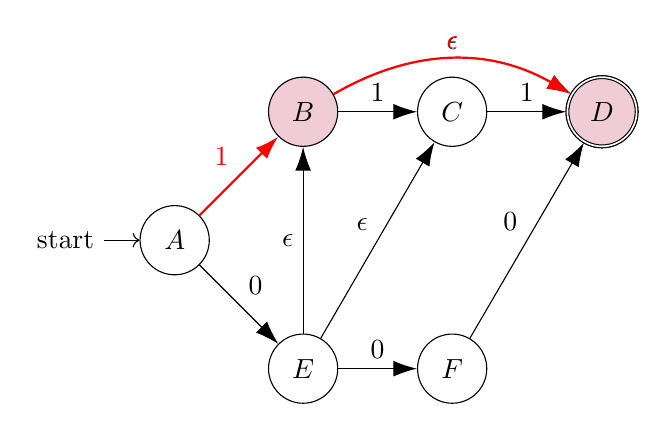
\begin{tikzpicture}[auto,
    ->,
    -{Latex[length=3mm,width=2mm]}
  ]
    \node[initial, state]   (a)                {$A$};
    \node[state] (b) [above right = of a, fill=Pink!20] {$B$};
    \node[state] (c) [right = of b] {$C$};
    \node[state, accepting] (d) [right = of c] {$D$};
    \node[state] (e) [below right = of a] {$E$};
    \node[state] (f) [right = of e] {$F$};    
    \path (a) edge[Red, thick] node {$1$} (b)
          (a) edge node {$0$} (e)
          (b) edge node {$1$} (c)
          (b) edge[bend left] node {$\epsilon$} (d)
          (c) edge node {$1$} (d)
          (e) edge node {$\epsilon$} (b)
          (e) edge node {$\epsilon$} (c)
          (e) edge node {$0$} (f)
          (f) edge node {$0$} (d)
    ;

\pause
    \node[state, accepting, fill=Pink!20] (d) [right = of c] {$D$};
    \path (b) edge[Red, thick, bend left] node {$\epsilon$} (d)
    ;

  \end{tikzpicture}
}

\vspace{1cm}
\textbf{Input:} ${\color{Red}\textbf{1}}...$

\end{center}

\end{frame}
% frame end %%%%%%%%%%%%%%%%%%%%%%%%


% frame begin %%%%%%%%%%%%%%%%%%%%%%%%
\begin{frame}{Simulation of NFAs}
{$\epsilon$-closure}
\myminorheader{Example 2.2}
\begin{center}
\resizebox{!}{0.35\textheight}{%
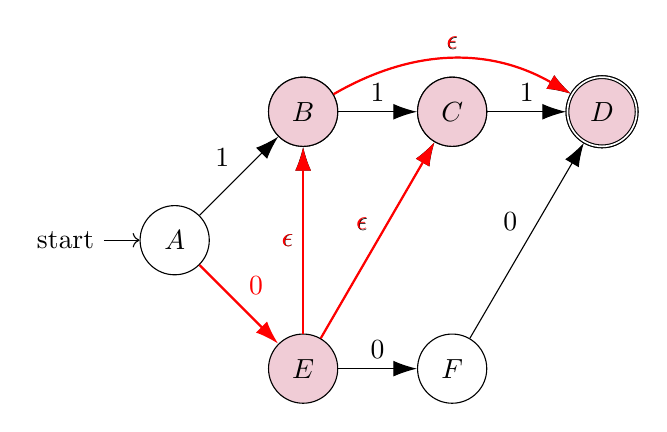
\begin{tikzpicture}[auto,
    ->,
    -{Latex[length=3mm,width=2mm]}
  ]
    \node[initial, state]   (a)                {$A$};
    \node[state] (b) [above right = of a] {$B$};
    \node[state] (c) [right = of b] {$C$};
    \node[state, accepting] (d) [right = of c] {$D$};
    \node[state, fill=Pink!20] (e) [below right = of a] {$E$};
    \node[state] (f) [right = of e] {$F$};    
    \path (a) edgenode {$1$} (b)
          (a) edge[Red, thick] node {$0$} (e)
          (b) edge node {$1$} (c)
          (b) edge[bend left] node {$\epsilon$} (d)
          (c) edge node {$1$} (d)
          (e) edge node {$\epsilon$} (b)
          (e) edge node {$\epsilon$} (c)
          (e) edge node {$0$} (f)
          (f) edge node {$0$} (d)
    ;

\pause
    \node[state, fill=Pink!20] (b1) at (b) {$B$};
    \node[state, fill=Pink!20] (c1) at (c) {$C$};
    \path (e) edge[Red, thick] node {$\epsilon$} (b)
		(e) edge[Red, thick] node {$\epsilon$} (c)
    ;
\pause
    \node[state, accepting, fill=Pink!20] (d) [right = of c] {$D$};
    \path (b) edge[Red, thick, bend left] node {$\epsilon$} (d)
    ;

  \end{tikzpicture}
}

\vspace{1cm}
\textbf{Input:} ${\color{Red}\textbf{0}}...$

\end{center}

\end{frame}
% frame end %%%%%%%%%%%%%%%%%%%%%%%%

% frame begin %%%%%%%%%%%%%%%%%%%%%%%%
\begin{frame}{Simulation of NFAs}
{$\epsilon$-closure}

\begin{itemize}
\item $\epsilon$-closure: computed on a set of states
\item Transitive closure of all states reachable through $\epsilon$-transitions
\item From a source state set $S_1$, on an input symbol $a$, the destination state set $S_2$ is computed as:

\begin{quotation}

$U = \bigcup\limits_{s \in S_1} Trans[s, a]$

%\vspace{0.5cm}

$S_2 = \epsilon \text{-closure}(U)$
\end{quotation}
\item $\epsilon$-closure -- a reflexive relation
\end{itemize}
\end{frame}
% frame end %%%%%%%%%%%%%%%%%%%%%%%%

% frame begin %%%%%%%%%%%%%%%%%%%%%%%%
\begin{frame}{Computing $\epsilon$-closure}
\footnotesize
\begin{algorithmic}[0]
\Procedure{$\epsilon$-closure}{$s$}
  \State $stack$.\Call{push}{$s$}
  \State $ep$.\Call{add}{$s$}
  \While{$stack$ is not empty}
    \State $t \gets stack$.\Call{pop}{}
    \State $U \gets \{u : u \in M.Trans[t, \epsilon]\}$
    \For{$u \in U$}
      \If{$u \notin ep$}
        \State $stack$.\Call{push}{$u$}
        \State $ep$.\Call{add}{$u$}
      \EndIf
    \EndFor
  \EndWhile
  \State \textbf{return} $ep$
\EndProcedure

\end{algorithmic}

\end{frame}
% frame end %%%%%%%%%%%%%%%%%%%%%%%%

% frame begin %%%%%%%%%%%%%%%%%%%%%%%%
\begin{frame}{Computing $\epsilon$-closure}
{Example}
\begin{center}
\resizebox{!}{0.3\textheight}{%
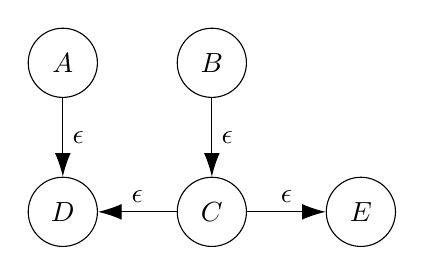
\begin{tikzpicture}[auto,
    ->,
    -{Latex[length=3mm,width=2mm]}
  ]
    \node[state] (A)                {$A$};
    \node[state] (B) [right = of A] {$B$};
    \node[state] (C) [below = of B] {$C$};
    \node[state] (D) [below = of A] {$D$};
    \node[state] (E) [right = of C] {$E$};
    
    \path 
          (A) edge node {$\epsilon$} (D)
          (C) edge node[above] {$\epsilon$} (D)
          (C) edge node {$\epsilon$} (E)
          (B) edge node {$\epsilon$} (C)
    ;
    
  \end{tikzpicture}
}

\vspace{1cm}

\begin{scriptsize}
\begin{tabular}{| l | l |}
\hline
\cellcolor{Gray!20}\color{Red}$ep$ & \cellcolor{Gray!20}\color{Red}$stack$ \\
\hline
& \\
\hline
\pause
$A$, $B$                & $B$, $A$  \\
\hline
\pause
$A$, $B$, $D$           & $B$, $D$ \\
\hline
\pause
$A$, $B$, $D$           & $B$ \\
\hline
\pause
$A$, $B$, $D$, $C$      & $C$ \\
\hline
\pause
$A$, $B$, $D$, $C$, $E$ & $E$ \\
\hline
\pause
$A$, $B$, $D$, $C$, $E$ &  \\
\hline

\end{tabular}
\end{scriptsize}
\end{center}
\end{frame}
% frame end %%%%%%%%%%%%%%%%%%%%%%%%

% frame begin %%%%%%%%%%%%%%%%%%%%%%%%
\begin{frame}{Simulating FSAs}

\myminorheader{Representating \textit{transition function} using transition tables}
\begin{center}
\resizebox{!}{0.2\textheight}{%
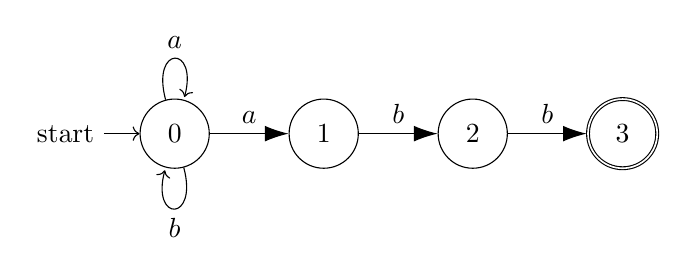
\begin{tikzpicture}[auto,
    ->,
    -{Latex[length=3mm,width=2mm]}
  ]
    \node[initial, state]   (0)                {$0$};
    \node[state]            (1) [right = of 0] {$1$};
    \node[state] (2) [right = of 1] {$2$};
    \node[state, accepting] (3) [right = of 2] {$3$};
    
    \path (0) edge[loop above] node {$a$} (0)
          (0) edge[loop below] node {$b$} (0)
          (0) edge node {$a$} (1)
          (1) edge node {$b$} (2)
          (2) edge node {$b$} (3)
    ;
    
  \end{tikzpicture}
}

\end{center}

\textbf{Transition Table:}
\begin{center}
\begin{tabular}{c | c | c }
\hline
\textbf{State} & \textbf{a}        & \textbf{b}     \\
\hline
\onslide<1->0              & \onslide<2->\{0, 1\}          & \onslide<2->\{0\} \\
\onslide<1->1              & \onslide<2->\{\}              & \onslide<2->\{2\} \\
\onslide<1->2              & \onslide<2->\{\}              & \onslide<2->\{3\} \\
\onslide<1->3              & \onslide<2->\{\}              & \onslide<2->\{\}
\end{tabular}
\end{center}
\end{frame}
% frame end %%%%%%%%%%%%%%%%%%%%%%%%

% frame begin %%%%%%%%%%%%%%%%%%%%%%%%
\begin{frame}{Simulation of NFA}
\begin{small}
\begin{algorithmic}[0]
\Procedure{simNFA}{$N$, $inp$}
\pause
  \State $S \gets$ \Call{$\epsilon$-closure}{$\{N.s_0\}$}
%  \State $c \gets$ \Call{nextChar}{}
  \While{there is input left}
    \State $c \gets$ \Call{nextChar}{}
    \State $T' \gets$ \Call{move}{$S$, $c$}
    \State $S \gets$ \Call{$\epsilon$-closure}{$T'$}
  \EndWhile
  \If{$S \cap N.F \neq \{\}$}
    \State \textbf{return true}
  \Else
    \State \textbf{return} \textbf{false}
  \EndIf
\EndProcedure
\end{algorithmic}
\end{small}

\pause
\begin{center}

\begin{tikzpicture}
\node[rectangle, draw=Red, fill=Red]{};
\end{tikzpicture}
\end{center}
\end{frame}
% frame end %%%%%%%%%%%%%%%%%%%%%%%%


% frame begin %%%%%%%%%%%%%%%%%%%%%%%%
\begin{frame}{Next}

\myheader{Conversion of NFA to DFA}
\end{frame}
% frame end %%%%%%%%%%%%%%%%%%%%%%%%

\end{document}
